\chapter{Results \& Discussion}
Results for radiation damage calculations and simulations are reported and discussed first, followed by results from TGS.

\section{Radiation damage}
In the absence of a dedicated monte carlo code to model the PbS(Th) thin film more accurately, quantifying the radiation damage requires some decisions about which sources of damage can be neglected. The 18.4 $\mu m$ range of alphas in PbS(Th) indicates that alphas traveling in the z-direction (the dimension in which the film is thin) traverse the 500 nm with little resistance and simply exit the sample. On the way, they disturb electrons and create phonons, but cause negligibly few displacements. This is true regardless of where in the sample they are born.

If, however, they are born with a trajectory in the xy plane (the dimensions in which the thin film is 1 cm x 1.5 cm), then the film is plenty large enough for them to deposit all of their energy and cause hundreds of displacements. However, the total solid angle for this situation is small compared with the solid angle of traversing the film in its thinner directions. In other words, most alphas will be born with a location and trajectory that leaves them very little PbS(Th) crystal to traverse before exiting the thin film.

The alpha energy used, 5423 keV, is of course, not the only alpha energy in the Th-228 decay chain. But it does represent the lowest energy/highest interaction alpha of the preferred alpha decays (the alpha which, for a particular nuclide, is emitted most often). As such, this analysis is even more true of the other, more energetic alphas in the decay chain.

This analysis has three important implications. 
\begin{itemize}
\item Damage from radiation with any lower probability of interaction can be neglected. This means gammas and betas, each with smaller interaction cross sections and less energy to deposit, can be neglected.
\item It justifies the assumption made earlier that all radiation produced by thorium decay chain is detectable. The alphas detected in the previous work by Templeman et al. faithfully represent the alphas born in the material, and the activity detected can be assumed to be the activity of the thorium decay chain.
\item The bulk of the radiation damage in the thin film must be a result of recoiling daughters.
\end{itemize}


\section{Thermal diffusivity and SAW speed}
Results are plotted in Figures \ref{thermal_diffusivity_pre_post}, \ref{curve_fit}, \ref{T_P_alpha_subplots}, and \ref{SAW_speeds}.  Figure \ref{thermal_diffusivity_pre_post} shows the thermal diffusivity over time for the duration of the experiment; thus indicating the baseline thermal diffusivity before annealing, and then the post-annealing baseline, followed by a monotonic increase over $\sim$4 hours. 

During the months preceding this experiment, radiation damage was presumed to reach a steady maximum. At this maximum, either the lattice would have become completely amorphous, or an equilibrium would exist whereby additional atomic displacements would be just as likely to create new Frenkel pairs as they would be to cause recombination.

Annealing was expected to heal the accumulated damage, allowing the whole process to begin again. One might expect that damage would \emph{reduce} thermal diffusivity, but that annealing would reset $\alpha$ to a \emph{higher} value associated with phonon transport in a low defect crystal. After annealing, the radiation damage would slowly set in, and TGS results would show the thermal diffusivity declining until it arrived back at the pre-annealing value. Or, if contrary to phonon scattering considerations, radiation damage actually \emph{increased} thermal diffusivity, then annealing would reset it to a \emph{lower} value and TGS would measure radiation damage increasing it. Regardless of what annealing might do to thermal diffusivity, we would expect radiation damage to push thermal diffusivity back to its pre-annealed value.

In brief, these intuitions amount to five primary expectations:
\begin{enumerate}
\item Radiation damage effects over the months preceding this work should have reached a steady state. Each parameter ought to be at an extremum.
\item Annealing should restore each parameter to its pre-irradiation value.
\item Radiation damage should tend to push the parameter back to its steady state value---the value measured prior to annealing.
\item Radiation damage should decrease thermal diffusivity
\item Radiation damage should decrease SAW speed.
\end{enumerate}

Neither thermal diffusivity nor SAW speed behaved entirely as expected.

Refer again to Figure \ref{SAW_speeds}. The data indicates that SAW speed is increased by radiation damage rather than decreased, but the rest of its behavior roughly matches expectation. Annealing pulls SAW speed down, and new radiation damage pushes SAW speed back toward its pre-annealing value.

There is in fact precedent in the literature for this behavior, even if it was not apparent that it was applicable before. In Dienes's 1952 paper and in Nabarro's response, the effect of interstitials and vacancies on elasticity is investigated \cite{Dienes1952a, Nabarro1952}. They conclude that vacancies exert a tensile stress on the material, while interstitials exert a compressive stress. These contributions are not equal and opposite, because interstitials exert an order of magnitude more stress \cite{Dienes1952a}. Their work on metals such as copper and sodium would at first seem not to be applicable because metallic bonds dictate very different response to radiation damage than the covalent bonds present in lead sulfide, but it amounts to a very compelling hypothesis for the results obtained in this work. Perhaps, then, the apparent increase in the maximum SAW speed (as a result of damage) after annealing is due to residual interstitials that did not recombine during annealing. Instead, the atoms around them relaxed, as Dienes describes, which effectively ``bakes'' in the damage. On the second round of radiation, damage and thus stiffness have a head start.

Refer again to Figure  \ref{thermal_diffusivity_pre_post}. The data indicates that annealing increases thermal diffusivity, but so does radiation damage. Since we expected the effect of annealing and the effect of radiation damage to cancel one another, this is very surprising. It is also not clear how the thermal diffusivity got so low as its pre-annealing value if months of radiation damage should have increased it.

Of the two competing mechanisms discussed in the background---increased charge carrier mobility and increased phonon scattering---the data appears to suggest that increased charge carrier mobility is actually dominant effect of radiation damage. Or, at least it does in the short term. There could be both short term and long term effects that are opposing. This could explain the increase in thermal diffusivity over this experiment, while also accounting for a gradual decline months later when the latent effect takes over.

As a final note, in both samples we observe a ``hook'' before the overall post-annealing trend emerges. Since the timing of the hook behavior lines up with the times the chamber was cracked to atmosphere and then re-pumped (see \ref{T_P_alpha_subplots}), it is believe that this behavior is a result of the pressure differential, and not radiation damage. We already know that lead sulfide's band gap is sensitive to pressure, so it makes sense that its other properties would be too. For the purposes of this study, we can treat as comparable only the TGS measurements taken below 15 mTorr.


%Mike Short recommends these:
%G. J. Dienes, A theoretical estimate of the effect of radiation on the elastic constants of simple metals, Phys. Rev. 86, 228 (1952).
%F. R. N. Nabarro, Effect of radiation on elastic constants, Phys. Rev. 87, 665 (1952).
%G. J. Dienes, Effect of radiation on elastic constants, Phys. Rev. 87, 666 (1952).


% hook
% New energy levels in the gap
% Umklapp scattering
% Phonon scattering off defects
% heat? pressure?
% 1) messed up analysis
% 2) messed up experiment
% 3) Annealing problem
% 		delamination, atoms boiling off, phase transition, oxidation, change in grain size
% 4) pressure problem
% 5) 

% why not short term mobility + long term phonon scattering?
% curve is exponential
% resistance should have diminished.



\begin{figure}[pt]
\begin{center}
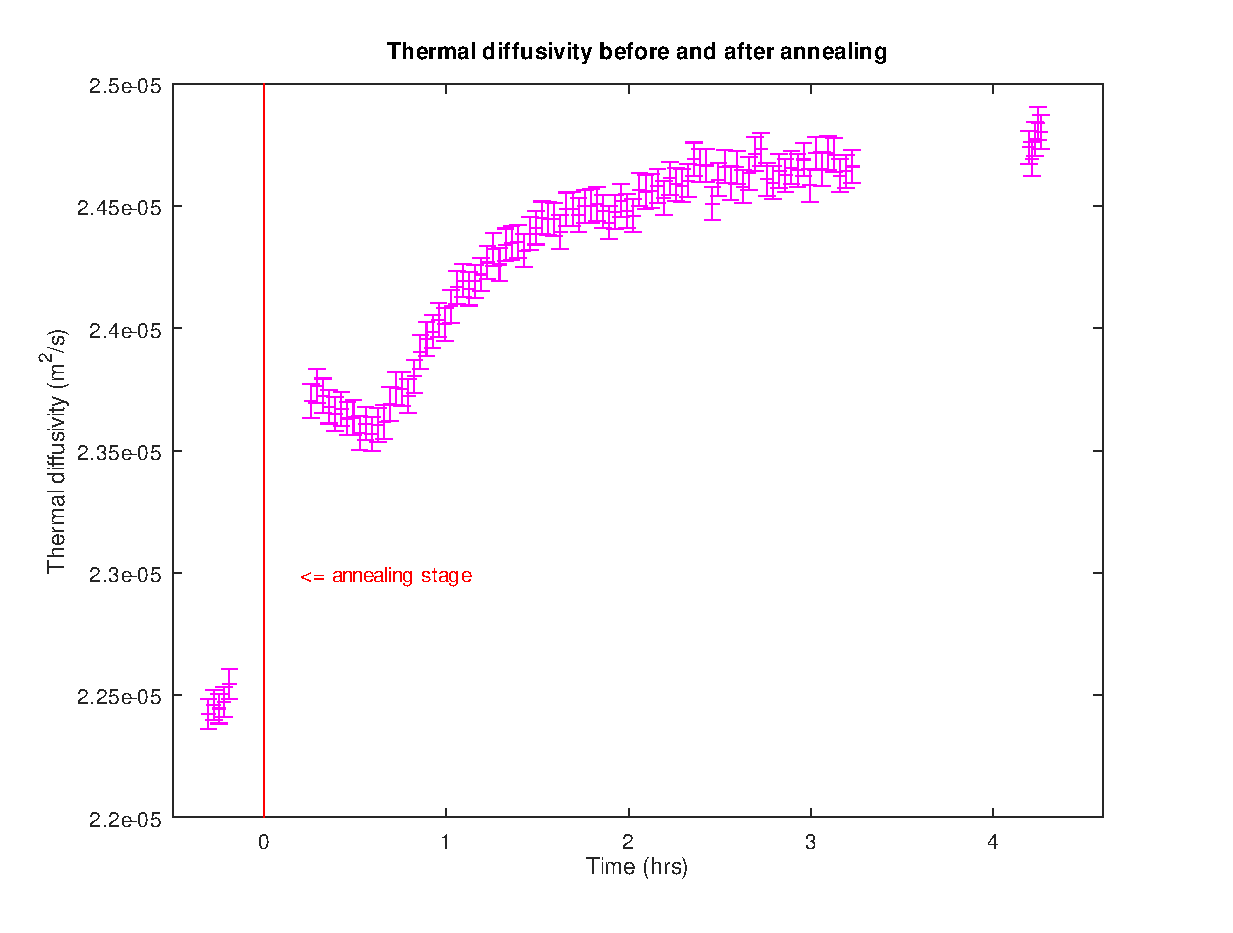
\includegraphics[width=\textwidth]{./images/thermal_diffusivity_pre_post.eps}
\caption{Thermal diffusivity results from TGS for entire experiment. Annealing stage is cut out for ease of comparing pre-annealing thermal diffusivity values (left of the red line) to post-annealing thermal diffusivity values (right of the red line). As radiation damage events per second are constant over the experiment, damage accumulates linearly with elapsed time since annealing.}
\label{thermal_diffusivity_pre_post}
\end{center}
\end{figure}

\begin{figure}[pt]
\begin{center}
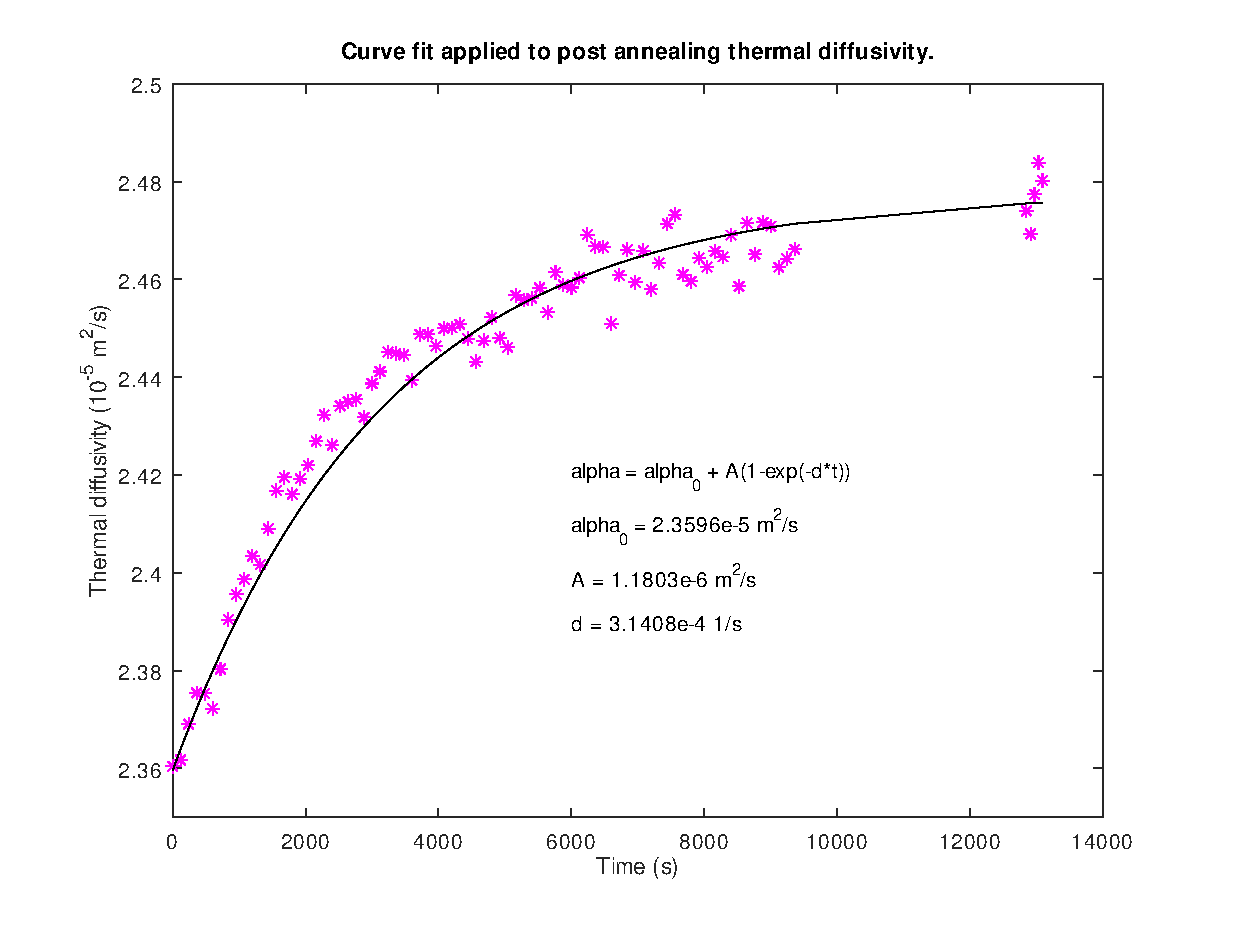
\includegraphics[width=\textwidth]{./images/curve_fit.eps} 
\caption{Generalized least squares fit to thermal diffusivity data after annealing and after ``hook''. Equation form chosen due to evidence that damage approaches a maximum.}
\label{curve_fit}
\end{center}
\end{figure}


\begin{figure}[pt]
\begin{center}
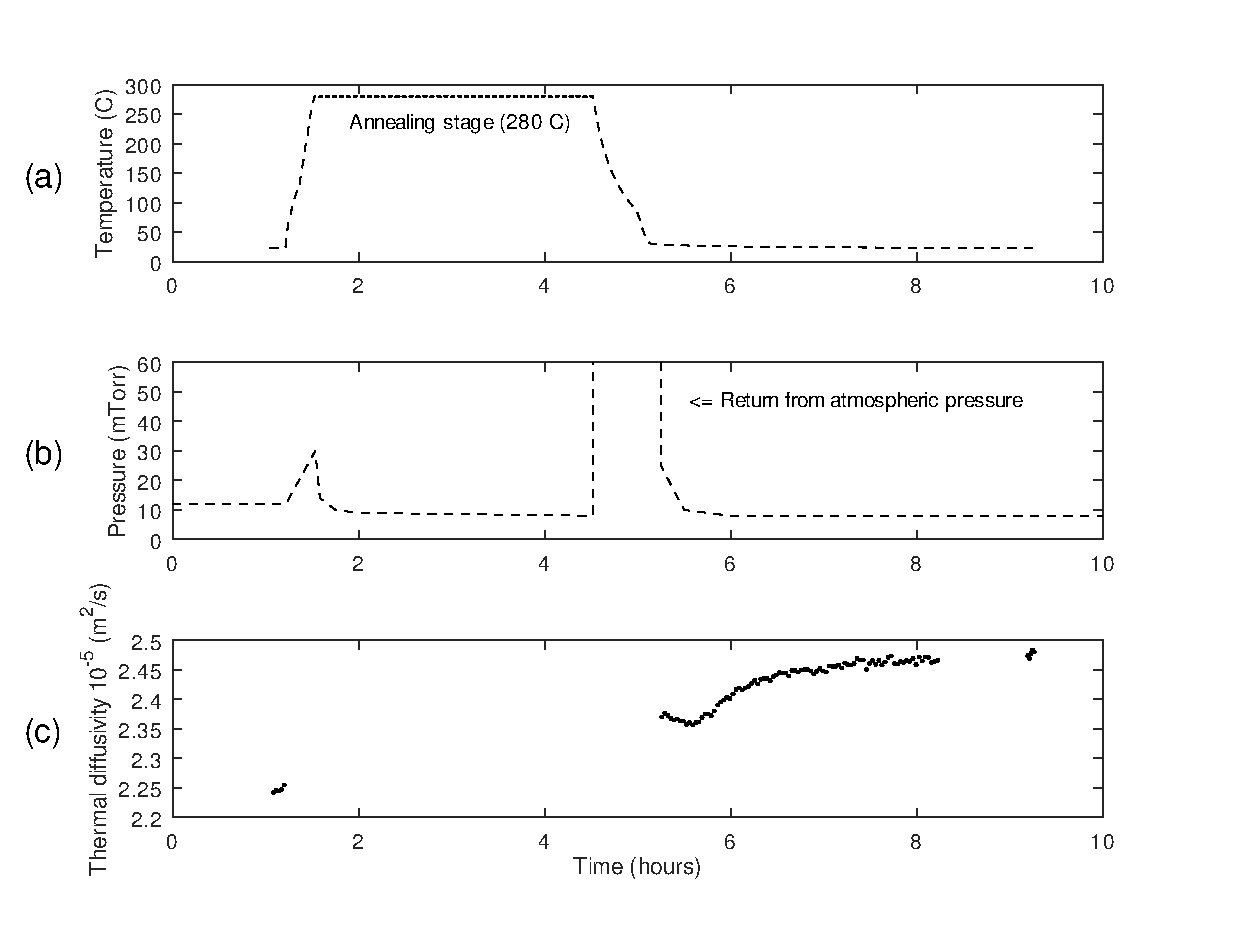
\includegraphics[width=\textwidth]{./images/T_P_alpha_subplots.eps}
\caption{Thermal diffusivity results from TGS are again plotted for the entire experiment in (c), but this time accompanied by the temperature record in (a) and the pressure record in (b) to clarify chronology of experiment. This also illustrates the coincidence between the pressure transient and the hook in the post-anneal thermal diffusivity data at $\sim$5.5 hours.}
\label{T_P_alpha_subplots}
\end{center}
\end{figure}


\begin{figure}[pt]
\begin{center}
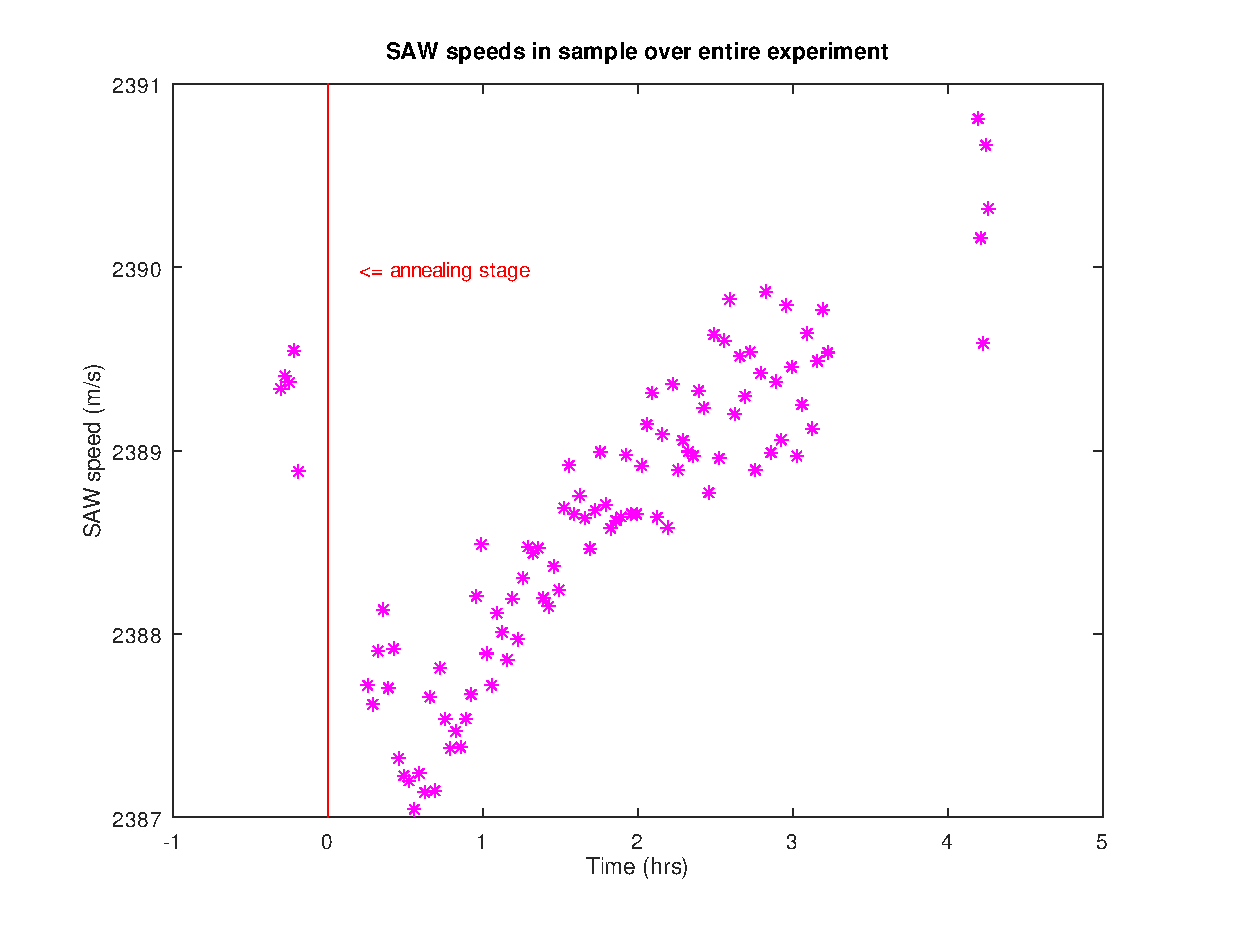
\includegraphics[width=\textwidth]{./images/SAW_speeds.eps}
\caption{SAW speed results from TGS are plotted for the entire experiment. The annealing stage is cut out so that pre and post annealing measurements can be compared more easily by eye. As SAW speed is proportional to elasticity, this plot indicates that annealing reduces stiffness caused by radiation damage, which immediately begins to accumulate again.}
\label{SAW_speeds}
\end{center}
\end{figure}




% \cite{patterson:risc,rad83}.  
% \cite{ellis:bulldog,pet87,coutant:precision-compilers}.  In these cases, the
% \cite{gib86}.
% These optimizations are described in detail in section~\ref{ch1:opts}.
% \section{Description of micro-optimization}\label{ch1:opts}
% \footnote{A description of the floating point format used is shown in figures~\ref{exponent-format}
% and~\ref{mantissa-format}.}.  
% A discussion of the mathematics behind unnormalized arithmetic is in appendix~\ref{unnorm-math}.

% \footnote{Using unnormalized numbers for math is not a new idea; a
% good example of it is the Control Data CDC 6600, designed by Seymour Cray.
% \cite{thornton:cdc6600} The CDC 6600 had all of its instructions performing
% unnormalized arithmetic, with a separate {\tt NORMALIZE} instruction.}.

% This is an example of how you would use tgrind to include an example
% of source code; it is commented out in this template since the code
% example file does not exist.  To use it, you need to remove the '%' on the
% beginning of the line, and insert your own information in the call.
%
%\tagrind[htbp]{code/pmn.s.tex}{Post Multiply Normalization}{opt:pmn}

% This is an example of how you would use tgrind to include an example
% of source code; it is commented out in this template since the code
% example file does not exist.  To use it, you need to remove the '%' on the
% beginning of the line, and insert your own information in the call.
%
%\tgrind[htbp]{code/be.s.tex}{Block Exponent}{opt:be}
